% ---------------Grundeinstellungen---------------------------------------------------------
\documentclass[a4paper,12pt, DIV12]{scrartcl}
% Trennungen, Schriftsatz; neue Deutsche Rechtschreibung
\usepackage[ngerman]{babel}
\usepackage{lmodern,dsfont} % Modernere Version der Standard-Schriftart

\usepackage[utf8x]{inputenc}
\usepackage[T1]{fontenc} % Umlaute, Sonderzeichen...
%-----------------------------------------------------------------------------------------

%------------------Packete----------------------------------------------------------------
% Paket um Grafiken einzubinden. Evtl. muss unter Windows
% mit \usepackage[dvips]{graphicx} der dvips-Treiber für EPS-Grafiken
% geladen werden
\usepackage{graphicx}
\usepackage{subfigure}  % Bilder platzieren(z.B. nebeneinander)
\usepackage{multicol} % Paket für mehrspaltige Dokumente
\usepackage{float}    % Paket um Bilder in Fliess-Umgebungen einzubinden
\usepackage{amsmath}  % stellt die align-Umgebung zum Einrücken von Formeln zu Verfügung
\usepackage{amssymb}  % Extra mathematische Symbol
\usepackage{mathabx}  % für vernünftiges :=
\usepackage{amsthm}   % für q.e.d-Symbol
\usepackage{color}    % Farbdefinitionen
\usepackage{hyperref} % fuer klickbare Links
\usepackage{lastpage} % Spezielles Paket um die Seiten zu zählen
\usepackage{scrpage2} % Kopf- und Fusszeilen
\usepackage{enumerate} % Aufzählungen
%\usepackage{listings} % Quellcode farbig darstellen
%\usepackage{pst-circ} % Elektronische Schaltungen
%\usepackage{pgfplots} % Für Diagramme

%----------------------------------------------------------------------------------------

%----------------Konfiguration-----------------------------------------------------------
\ihead{Inoffizielles Script zur Vorlesung Algebra 1 WS 2011, Prof. Schmidt}
%\chead{}
\ohead{Seite \thepage}
%\ifoot{}
\ofoot{Stand: \today}
%\cfoot{}
%\pagemark = Seitenzahl
\setheadsepline{1pt}    % Dicke der Trennlinie Kopfzeile - Text
\setfootsepline{0.5pt}  % Dicke der Trennlinie Fusszeile - Text
\pagestyle{scrheadings} % gemachte Einstellungen anwenden
\usepackage{setspace}   % Linienabstand
\onehalfspacing         % 1.5 Zeilenabstand; 1 = \singlespacing; 2 =
% \doublespacing
% schönere Hyperlinkfarben
\definecolor{darkred}{rgb}{0.5,0,0}
\definecolor{darkgreen}{rgb}{0,0.5,0}
\definecolor{darkblue}{rgb}{0,0,0.5}
\hypersetup{
  colorlinks,
  linkcolor=darkblue,
  filecolor=darkgreen,
  urlcolor=darkred,
  citecolor=darkblue
}
% Absatzeinzug
\setlength{\parindent}{0pt}  % Kein Einzug der ersten 1.Zeile eines Absatzes
% Verzeichnis in dem nach Bildern gesucht wird
% Sollte laut Dokumentation auch unter Windows/Mac gehen. Kann das jemand bestätigen?
\graphicspath{{bilder/}{:bilder:}}
%----------------------------------------------------------------------------------------

%-------------------------------Befehlsdefinitionen--------------------------------------
\newcommand{\Pot}{\mathcal P}

\newcommand{\Def}{\text{Def}}
\newcommand{\Wert}{\text{Wert}}

\newcommand{\Abb}{\text{Abb}}
\newcommand{\Map}{\text{Map}}

\newcommand{\Inj}{\text{Inj}}
\newcommand{\Surj}{\text{Surj}}
\newcommand{\Bij}{\text{Bij}}

\newcommand{\ggT}{\text{ggT}}
\newcommand{\kgV}{\text{kgV}}

\newcommand{\supp}{\text{supp}}
%----------------------------------------------------------------------------------------

%----------------Beginn des eigentlichen Dokuments(also des Inhalts)---------------------
\begin{document}
\begin{titlepage}
\title{Inoffizielles Script zur Vorlesung Algebra 1 WS 2011 für IST, Prof. Schmidt}
% CS: Ich habe einfach mal die git Namen verwendet. Wer nicht drin stehen will, löscht sich halt wieder raus.
% Wir können auch Realnamen nehmen wenn ihr wollt. Meine commits sind ja eh immer mit dem vollen Namen ...
\author{Mitwirkende Autoren:\\
Mic92
\\
chaosbastler
\\
js75
}
\date{Revision: \today}
\maketitle

\begin{abstract}
Dieses Script wird fortlaufend mit den Vorlesungen erweitert. Es lohnt sich also ab und an nach Updates zu schauen.
\\Mitarbeit ist natürlich erwünscht, weitere Informationen auf der Projektseite: \url{https://github.com/Mic92/Algebra-I}
\end{abstract}
\end{titlepage}

\newpage
\tableofcontents
\newpage
\section{Mengen}
\input{mengen/grundlegendes.tex}
\newpage
\subsection{Mächtigkeit von Mengen}
Für endliche (abzählbare) Mengen ist die Mächtigkeit gleichzusetzen mit der Anzahl
der Elemente einer Menge. Für unendliche (nicht abzählbare) Mengen müssen andere
Definitionen getroffen werden, um deren Mächtigkeit zu beschreiben.
\paragraph{Man schreibt:}
\({}|{}A{}|{}\) oder \(\#A\)
\paragraph{Es gilt:}
\begin{math}
{}|{}2^A{}|{} = 2^{{}|{}A{}|{}}
\end{math}

\paragraph{Satz von Cantor}
Die Mächtigkeit der Potenzmenge einer Menge A ist stets größer als die Mächtigkeit der Menge A selber:
$$ |2^A| > |A| $$
Dies gilt insbesondere für die leere Menge, da $2^0>0$.
Außerdem ist für sämtliche endliche Mengen klar: $ 2^n > n $.  Auch bei unendlichen Mengen lässt sich die Gültigkeit des Satzes zeigen.

\subsubsection*{Gleichmächtigkeit}
Seien A und B zwei beliebige Mengen.
Dann heißt A gleichmächtig zur Menge B, wenn eine Bijektion (\({f:A}\rightarrow{B}\)) gebildet
werden kann. Das bedeutet, dass eine Vorschrift existiert, welches
jedem Element der Menge A genau ein Element der Menge B zuordnet.
Dabei werden alle Elemente der Menge B einmal erfasst. Diese
Vorschrift ist umkehrbar.
\paragraph{Man schreibt:} \(\#A = \#B\) bzw. \(|A| = |B|\)
\paragraph*{Beispiele:}
\begin{math}
\#{\mathbb N} = \#{\mathbb Z} = \#{\mathbb Q}
\end{math}

Jede Menge, die gleichmächtig zur Menge der natürlichen Zahlen ist, wird als \emph{abzählbar} bezeichnet.
Die Mächtigkeit der reelen Zahlen hingegen wird als \emph{überabzählbar} bezeichnet.
\subparagraph{Erläuterung zu \(\#{\mathbb N} = \#{\mathbb Z}\):}
\begin{figure}[b]
  \centering
  \caption{Beispiel für eine Abbildung \(\#{\mathbb N} = \#{\mathbb Z}\)}
  \includegraphics[scale=0.5]{ngleichz.pdf}
\end{figure}
Der Einwand, dass die natürlichen Zahlen doch ``offensichtlich'' (von der 0
abgesehen) doppelt so viele seien müssten, wie die ganzen Zahlen zählt
bei diesen unendlichen Mengen nicht! Stattdessen sollte man an die
Definition der Gleichmächtigkeit denken: 2 Mengen sind dann gleich,
wenn es eine eineindeutige(bijektive) Abbildung gibt.
Es werden also die 0 auf die 0, die ungeraden Zahlen auf die positiven
Zahlen und die geraden Zahlen auf die negativen Zahlen abgebildet.
Dies ist aufgrund der Unendlichkeit der beiden Mengen ohne Probleme
möglich.

Auch für die rationalen Zahlen lässt sich ein solches Schema für eine Bijektion finden.
Hierauf geht ein Wikipedia-Artikel näher ein:

% J.S.: Wir sollten die Wikipedia-Artikel später in das Skript einarbeiten..
\url{http://de.wikipedia.org/wiki/Cantors_erstes_Diagonalargument}

Und auch bei der Frage, warum die reellen Zahlen nicht abzählbar sind, hilft Wikipedia:

\url{http://de.wikipedia.org/wiki/Cantors_zweites_Diagonalargument}

% Quelle für nächsten Abschnitt: Repetorium höhere Mathematik, Merziger, Wirt, 6. Auflage, S.41 Aufgabe 1.60 und Lösung dazu
\subparagraph{Beispiel für überabzählbare Mengen}
Ähnlich wie beim vorherige Beispiel widerspricht es auch der Intuition, dass die Menge $\{ x | x \in (0,1) \}$ sowie $\{x | x \in {\mathbb R} \}$ gleichmächtig sind.
Schließlich ist das Intervall $(0,1)$ ja nur eine Teilmenge der reelen Zahlen.
\\Tatsächlich kann man schon mit Schulmathematik eine solche Bijektion finden: $$ f(x) = {1}/{\pi} * (arctan(x) + \pi/2 ) $$
Wer einen Blick auf den Graphen von $arctan(x)$ wirft wird dies schnell einsehen: 
die Funktion durchläuft sämtliche Werte von $-\infty$ bis $\infty$ und nimmt dabei nur Werte von $-\pi/2$ bis $\pi/2$ an. 
Durch Stauchung mit dem Faktor ${1}/{\pi}$ sowie Verschiebung nach oben kommt man dann zu obiger Funktion.

%%% Local Variables:
%%% mode: latex
%%% TeX-master: "../script"
%%% End:


\newpage
\section{Abbildungen}
\input{abbildungen/definition.tex}
\newpage
\subsection{Kern einer Funktion}
Sei $f:{A}\longrightarrow{B}$ eine Abbildungsvorschrift.
Dann ist die Menge
\begin{align*}
   \ker(f) := \{(a,b) | f(a)=f(b)\} %Interessant: \ker ist bereits definiert!
\end{align*}
der sogenannte Kern von f.
Umgangssprachlich ausgedrückt: Alle Paare, die den selben Funktionswert besitzen.
\subsubsection{Beispiel}
\begin{align*}
  f: &\mathbb{R} \rightarrow \mathbb{R} : {x}\longmapsto{x^2} \\
  \ker(f) &= \{(a,b) | f(a)=f(b) \} \\
         &= \{ (a,b) | a^2 = b^2 \} \\
         &= \{ (a,b) | |a| =|b| \}
\end{align*}
Ein anschaulicher Erklärungsversuch: Um den Kern dieser Funktion zu bestimmen, zeichnet man eine Parallele zur X-Achse zum Graph der Funktion(vgl. Grafik).
Nun untersucht man an der Stelle a, welche Werte den den selben Funktionswert besitzen. Offensichtlich trifft die Parallele zur X-Achse den Graph wiederrum bei -a. 
Also muss die Menge $\{(0,0),(1,-1),(-1,1),(2,-2), ...\} = \{ (a,-a) | a \in \mathbb{R} \}$ Teil des Kerns sein.
Außerdem muss(wie unter \ref{kern_eigenschaften} erläutert wird) auch die Menge $\{(a,a) | a \in \mathbb{R} \}$ im Kern enthalten sein, was insgesamt zu obigem Ergebnis führt. 
\begin{center}
 \includegraphics[keepaspectratio=true]{../bilder/parabel_kernsvg.pdf}
 % parabel_kernsvg.pdf: 194x166 pixel, 72dpi, 6.84x5.86 cm, bb=0 0 194 166
\end{center}

\subsubsection{Rechnerische Behandlung}
Je nach Abbildung kann man den Kern auch rechnerisch bestimmen. Hierfür soll das Beispiel noch einmal etwas ausführlicher erläutert werden.
Der Ausgangspunkt ist, dass zwei (nicht notwendigerweise verschiedene) Werte $x_1, x_2$ auf das selbe Element abgebildet werden sollen:
$$  f(x_1) = f(x_2) $$
$$ {x_1}^2 = {x_2}^2$$
Wurzelziehen führt zu den Lösungen
$ x_1 = x_2 $ sowie $ x_1 = - x_2 $
Dieses Beispiel ist rechnerisch recht trivial, entscheident ist, dass man den Ansatz verstanden hat: 
man muss für (möglicherweise unterschiedliche) Werte beim Einsetzen in die Funktion das selbe Ergebnis erhalten.
\footnote{Wenn gewünscht, kann man hier auch ein etwas komplexeres Beispiel (so wie das in der Übung z.B.) einfügen. Sagt einfach irgendwie Bescheid, wenn Bedarf besteht.}


\subsubsection{Eigenschaften des Kerns}\label{kern_eigenschaften} 
Wegen $ f(a) = f(a) $ muss $\ker(f)$ immer $\{(a,a) | a \in {A} \}$ enthalten.
Anders formuliert: da man bei einer Funktion für ein und den selben Eingabewert immer das selbe herrausbekommt, müssen diese im Kern enthalten sein.

% Brauch mein Emacs um das Masterfile zu finden
%%% Local Variables:
%%% mode: latex
%%% TeX-master: "../script"
%%% End:

\newpage
%*********************************************************%
% 17.11 : Alte Definitionen wieder hergestellt. (chaosbastler)
%*********************************************************
\subsection{Typen von Abbildungen}\label{kap_typabb}
\subsubsection{Definition}

\begin{figure}
\subfigure[surjektive
Abbildung]{\includegraphics[width=3cm]{Surjection.pdf}}\hfill
\subfigure[injektive
Abbildung]{
\includegraphics[width=3cm]{Injection.pdf}}\hfill
\subfigure[bijektive
Abbildungen]{\includegraphics[width=3cm]{Bijection.pdf}}\hfill
\subfigure[identische
Abbildungen]{
\includegraphics[width=3cm]{Identitaet.pdf}}
\end{figure}


Seinen A und B zwei Mengen und $f:{A}\longrightarrow{B}$ eine Abbildungsvorschrift.
Dann gibt es 3 besondere Typen von Abbildungen:
\begin{description}
\item[surjektive Abbildung] \emph{alle} Elemente von B mindestens einmal erfassen
$$ \forall b \in B \exists a \in A : f(a)=b $$
\item[injektive Abbildungen] alle Elemente von A erhalten \emph{unterschiedliche} Elemente aus B  (''keine Kollisionen``)
$$ \forall a_1,a_2  \in A : f(a_1)=f(a_2) \Rightarrow a_1 = a_2 $$
\item[bijektive Abbildungen] \emph{surjektiv und injektiv} zu gleich: alle A erhalten genau ein B und alle B werden getroffen.
Dies impliziert die Umkehrbarkeit der Funktion. Eine Sonderform der bijektiven
Abbildung ist die \emph{Identität}. Dabei wird jedes Element sich selbst zugeordnet.
$$ \forall b \in B \exists ! a \in A : f(a) = b $$
\end{description}

Ist $f \colon A \rightarrow B$ eine Abbildung, so sei für $X \subseteq A$ stets
$fX \coloneq f[X] \coloneq \{fx | x \in X\}$ die Menge der Bilder von $X$ unter
$f$.
Ferner heiße $\text{Bild}(f) = \text{Im}(f) \coloneq fA$ die
\emph{Bildmenge}\footnote{Bild = Image} von $f$. $f$ ist genau dann surjektiv,
wenn (gdw\footnote{im englischen Sprachraum \emph{iff} = if and only if}) $fA = B$
gilt, das heißt die Bildmenge von $f$ ist gleich der Zielmenge von $f$. Daraus
folgt: $fX \subseteq fA$

\newpage

\subsubsection{Bezeichnungen}
\begin{description}
\item Sind $A$ und $B$ Mengen, so bezeichnen $B^A \coloneq \text{Abb}(A,B)
\coloneq \Map(A,B)$ die Menge aller Abbildungen von $A$ nach $B$.
\item $\Surj(A,B)$ sei die Menge aller surjektiven Abbildungen
(\emph{Surjektionen}) von $A$ nach $B$,
\item $\Inj(A,B)$ sei die Menge aller injektiven Abbildungen
(\emph{Injektionen}) von $A$ nach $B$,
\item $\Bij(A,B)$ sei die Menge aller bijektiven Abbildungen
(\emph{Bijektionen}) von $A$ nach $B$.
\end{description}


\subsubsection{Mächtigkeit von Definitions- und Wertebereich}

Für Surjektionen gilt: $|A| \geq |B|$

Für Injektionen gilt: $|B| \geq |A|$

Weil für bijektive Abbildungen beide Aussagen gelten müssen gilt:
$$|A| \geq |B| \wedge |B| \geq |A| \Rightarrow |A| = |B| $$


Analog gilt auch:
$$ |A|<|B| \Longleftrightarrow \Surj(A,B) = \emptyset $$
$$ |A|>|B| \Longleftrightarrow \Inj(A,B) = \emptyset $$
$$ |A| \neq |B| \Longleftrightarrow \Bij(A,B) = \emptyset $$

Die ersten Aussagen schließen von einem Typ von Abbildung auf die Mächtigkeit von Definitions- und Wertebereich.
Die drei letzen Aussagen schließen von Definitions- und Wertebereich auf die (nicht) möglichen Typen von Abbildungen.

Würden die Beziehungen zwischen den Mächtigkeiten nicht gelten, würde z.B. die
Formel zur Mächtigkeit von $\Inj(A,B)$ zu Widersprüchen führen(vlg. nächstes
Kapitel).

\newpage
\subsection{Mächtigkeit von Mengen}
Für endliche (abzählbare) Mengen ist die Mächtigkeit gleichzusetzen mit der Anzahl
der Elemente einer Menge. Für unendliche (nicht abzählbare) Mengen müssen andere
Definitionen getroffen werden, um deren Mächtigkeit zu beschreiben.
\paragraph{Man schreibt:}
\({}|{}A{}|{}\) oder \(\#A\)
\paragraph{Es gilt:}
\begin{math}
{}|{}2^A{}|{} = 2^{{}|{}A{}|{}}
\end{math}

\paragraph{Satz von Cantor}
Die Mächtigkeit der Potenzmenge einer Menge A ist stets größer als die Mächtigkeit der Menge A selber:
$$ |2^A| > |A| $$
Dies gilt insbesondere für die leere Menge, da $2^0>0$.
Außerdem ist für sämtliche endliche Mengen klar: $ 2^n > n $.  Auch bei unendlichen Mengen lässt sich die Gültigkeit des Satzes zeigen.

\subsubsection*{Gleichmächtigkeit}
Seien A und B zwei beliebige Mengen.
Dann heißt A gleichmächtig zur Menge B, wenn eine Bijektion (\({f:A}\rightarrow{B}\)) gebildet
werden kann. Das bedeutet, dass eine Vorschrift existiert, welches
jedem Element der Menge A genau ein Element der Menge B zuordnet.
Dabei werden alle Elemente der Menge B einmal erfasst. Diese
Vorschrift ist umkehrbar.
\paragraph{Man schreibt:} \(\#A = \#B\) bzw. \(|A| = |B|\)
\paragraph*{Beispiele:}
\begin{math}
\#{\mathbb N} = \#{\mathbb Z} = \#{\mathbb Q}
\end{math}

Jede Menge, die gleichmächtig zur Menge der natürlichen Zahlen ist, wird als \emph{abzählbar} bezeichnet.
Die Mächtigkeit der reelen Zahlen hingegen wird als \emph{überabzählbar} bezeichnet.
\subparagraph{Erläuterung zu \(\#{\mathbb N} = \#{\mathbb Z}\):}
\begin{figure}[b]
  \centering
  \caption{Beispiel für eine Abbildung \(\#{\mathbb N} = \#{\mathbb Z}\)}
  \includegraphics[scale=0.5]{ngleichz.pdf}
\end{figure}
Der Einwand, dass die natürlichen Zahlen doch ``offensichtlich'' (von der 0
abgesehen) doppelt so viele seien müssten, wie die ganzen Zahlen zählt
bei diesen unendlichen Mengen nicht! Stattdessen sollte man an die
Definition der Gleichmächtigkeit denken: 2 Mengen sind dann gleich,
wenn es eine eineindeutige(bijektive) Abbildung gibt.
Es werden also die 0 auf die 0, die ungeraden Zahlen auf die positiven
Zahlen und die geraden Zahlen auf die negativen Zahlen abgebildet.
Dies ist aufgrund der Unendlichkeit der beiden Mengen ohne Probleme
möglich.

Auch für die rationalen Zahlen lässt sich ein solches Schema für eine Bijektion finden.
Hierauf geht ein Wikipedia-Artikel näher ein:

% J.S.: Wir sollten die Wikipedia-Artikel später in das Skript einarbeiten..
\url{http://de.wikipedia.org/wiki/Cantors_erstes_Diagonalargument}

Und auch bei der Frage, warum die reellen Zahlen nicht abzählbar sind, hilft Wikipedia:

\url{http://de.wikipedia.org/wiki/Cantors_zweites_Diagonalargument}

% Quelle für nächsten Abschnitt: Repetorium höhere Mathematik, Merziger, Wirt, 6. Auflage, S.41 Aufgabe 1.60 und Lösung dazu
\subparagraph{Beispiel für überabzählbare Mengen}
Ähnlich wie beim vorherige Beispiel widerspricht es auch der Intuition, dass die Menge $\{ x | x \in (0,1) \}$ sowie $\{x | x \in {\mathbb R} \}$ gleichmächtig sind.
Schließlich ist das Intervall $(0,1)$ ja nur eine Teilmenge der reelen Zahlen.
\\Tatsächlich kann man schon mit Schulmathematik eine solche Bijektion finden: $$ f(x) = {1}/{\pi} * (arctan(x) + \pi/2 ) $$
Wer einen Blick auf den Graphen von $arctan(x)$ wirft wird dies schnell einsehen: 
die Funktion durchläuft sämtliche Werte von $-\infty$ bis $\infty$ und nimmt dabei nur Werte von $-\pi/2$ bis $\pi/2$ an. 
Durch Stauchung mit dem Faktor ${1}/{\pi}$ sowie Verschiebung nach oben kommt man dann zu obiger Funktion.

%%% Local Variables:
%%% mode: latex
%%% TeX-master: "../script"
%%% End:


\newpage
\section{Graphen}
\input{graphen/gerichteter_multigraph.tex}
\newpage
\input{graphen/binaere_relate.tex}
\newpage
\subsection{Morphismen zum Vergleich von Graphen}
\subsubsection{Definition}
Seien G und G' zwei Netzwerke(Graphen) sowie $G \overset{\Phi}{\rightarrow} G'$ 
\\Dann ist $\Phi  = (\Phi_{kante}, \Phi_{ecke})$  ein \emph{Morphismus} ein Paar von Abbildungen:
$$ \Phi_{vert}: V \rightarrow V'$$
$$\Phi_{edge}: E \rightarrow E'$$
mit $\tau' \Phi_{edge} e = \Phi_{vert} \tau e$
\\und $ {\sigma '}  \Phi_{edge} e = \Phi_{vert} \sigma e$
% Anmerkung: An der Tafel Stand nicht E -> E' sondern E->V'; im einer Zusammenfassung von Algebra im ET Forum stand diese Version. Was ist richtig?
\\D.h. das Bild des Anfangsknoten einer Kante e ist Anfangsknoten der Bildkante.
\paragraph{Merkregel}``Fuß und Kopf gehen nicht verloren''

\subsubsection{Beispiel}
\begin{figure}[h!]
 \subfigure[Netzwerk G]{  
\includegraphics[width=7cm]{../bilder/morphismus_bsp_a1.pdf} } \hfill
 % morphismus_bsp_a1.pdf: 652x369 pixel, 72dpi, 23.00x13.02 cm, bb=0 0 652 369
 \subfigure[Netzwerk G']{  
\includegraphics[width=5cm]{../bilder/morphismus_bsp_a2.pdf} }
 % morphismus_bsp_a2.pdf: 340x425 pixel, 72dpi, 11.99x14.99 cm, bb=0 0 340 425
\end{figure}
G und G' sind isomorph, man schreibt $G \cong G'$
%Bin mir nicht sicher ob das Beispiel nicht eventuell sogar noch weiter gehen könnte, so dass auch die einzelnen Elemente von G' z.B. anders heißen

\newpage
\section{Relationen}
% --Relationen--

\subsection{Eigenschaften}

Wenn $R \subseteq A \times A$ eine Relation ist, dann ist $R$:
\begin{itemize}
\item \emph{symmetrisch}, falls für $(a, b) \in \mathbb{R}$ stets auch
  $(b, a) \in \mathbb{R}$ gilt, z.B. Rechwinkligkeit: wenn $a \bot b$ ist,
  dann ist $b \bot a$.
 \item \emph{antisymmetrisch} falls für $(a, b) \in \mathbb{R}$ und $(b, a) \in \mathbb{R}$  stets folgt: $a \equiv b$
 \item \emph{reflexiv} falls $(a, a) \in \mathbb{R}$ für alle $a$ in
   $A$ gilt, z.B. Parallelität: Jede Gerade ist zu sich selbst parallel
 \item \emph{transitiv} falls aus $(a, b) \in \mathbb{R}$ und $(b, c)
   \in \mathbb{R}$ folgt: $(a, c) \in \mathbb{R}$, z.B. Kleiner-Gleich
   ``$\leq$'': Wenn $a \leq b$ und $b \leq c$, dann gilt $a \leq c$.
\end{itemize}

\subsection{Beispiel einer Relation: Teilbarkeit}

Seien $a, b \in \mathbb{N}$. Dann ist $a$ \emph{Teiler von} $b$ genau dann, wenn
es ein $m \in \mathbb{N}$ gibt, so dass gilt: $a \cdot m = b$.

\paragraph{Bezeichnung:} $a \mid b$, $a \le_\tau b$

\paragraph{Beispiel:}
\begin{align*}
3 \mid 6,                    & \text{ denn }     3 \cdot 2 = 6    \\
n \mid 0,                    & \text{ für alle } n \in \mathbb{N} \\
n \le_\tau 0,                 & \text{ für alle } n \in \mathbb{N} \\
0 \mid 0, \text{ } 0 \nmid k & \text{ für alle } k \in \mathbb{N} \setminus \{0\} \text{ (es gibt }  m \in \mathbb{N}: 0 \cdot m = 0 \text{)} \\
1 \mid n,                    & \text{ für alle } n \in \mathbb{N} \\
\end{align*}

\paragraph{Bemerkung:}
$\le_\tau$ ist eine Relation über $\mathbb{N}$:

$\le_\tau $ ist eine Untermenge von $\mathbb{N} \times \mathbb{N}$.

$(a,b) $ ist ein Element von $\le_\tau$, wenn gilt $a \le_\tau b$.



\noindent $T_n$ sei die Menge der Teiler von $n (n \in \mathbb{N})$. \\ \indent {\bf Beispiel:} $T_{12} = \{ 1, 2, 3, 4, 6, 12 \}$ \\

\noindent Wir schränken $\le_\tau$ ein auf $T_n$: $\le_\tau \cap (T_n \times T_n) = \le_\tau^n$

\paragraph{Konvention:} wir schreiben $\le_\tau$ statt $\le_\tau \cap (A \times A)$, wenn klar ist, worauf sich $\le_\tau$ bezieht, also was $A$ ist. \\

\noindent $\mathbb{T}_n := (T_n, \le_\tau)$ heißt {\bf Teilerverband} von $n$.

\paragraph{Achtung:} $\mathbb{T}_n$ ist ein binäres Relat. Wir haben
bereits definiert, was $G (\mathbb{T}_n) = G (T_n, \le_\tau)$ ist:
$G (\mathbb{T}_n) = (T_n, \le_\tau, \sigma, \tau) \text{ mit:}$
\begin{align*}
\sigma (a, b) = a\\
\tau (a, b) = b\\
\forall (a, b) \in \le_\tau
\end{align*}

\paragraph{Beispiel:} $\mathbb{T}_6 = (T_6, \le_\tau), T_6 = { 1, 2, 3, 6}$

Teilerverband $G (\mathbb{T}_6) $:
\begin{figure}[h]
  
\includegraphics[scale=0.5,keepaspectratio=true]{../bilder/teilerverband.pdf}
\end{figure}

\noindent Ist $R$ eine Ordnung über $A$, dann ist $G (A, R)$ eine ungünstige Darstellung. \\ {\bf Besser:} Hasse-Diagramm:

$\le_\tau$ ist eine Relation auf $\mathbb{N}$, die gegeben ist durch: \\
$ \le_\tau = \{ (a, b) \in \le_\tau | \text{ für alle } c \in \mathbb{N} \text{ mit } a \le_\tau c \le_\tau b, (a, c), (c, b) \in \le_\tau \text{ gilt entweder } c = a \text{ oder } c = b \}$

\paragraph{Beispiel:}
\begin{itemize}
\item $(1, 6) \in \le_\tau$, aber $1 \le_\tau 2 \le_\tau 6$ und
                                 $1 \le_\tau 3 \le_\tau 6$,
  daraus folgt $(1, 6) \not\in\le_\tau$.
 \item $(2, 6) \in \le_\tau$ und für alle $c \in T_6$ mit $2 \le_\tau c \le_\tau 6$ gilt $c = 2$ oder $c = 6 \rightarrow (2, 6)$
\end{itemize}

\paragraph{Hassediagramm zu $\mathbb{T}_n$:}

Zeichne $G (T_n, \le_\tau)$, so dass der Knoten b über dem Knoten $a$
liegt, falls $(a, b) \in \le_\tau$ und zeichne Kanten $(a, b)$, also
$a$ ----- $b$ statt $a \longrightarrow b$. \\

\begin{figure}[h]
  
\includegraphics[scale=0.5,keepaspectratio=true]{../bilder/hassediagramm_von_6.pdf}
  \includegraphics[keepaspectratio=true]{../bilder/hassediagramm_von_60.pdf}
  \caption{Hassediagramm vom Teilerverband 6 und 60}
\end{figure}

\subsection{Division mit Rest}

Die \emph{Division mit Rest} besagt, dass für 2 Zahlen $n$ und $m$
(ungleich 0) eindeutig bestimmte Zahlen $a$ und $b$ existieren für die gilt:
\begin{itemize}
\item $n = a * m + b$
\item $0 \le n < b$
\end{itemize}

Der Modulo berechnet den Rest $b$ der Division $n/m$. Schreibweise: $n \bmod a = b$

Beim Rechnen mit Modulo lassen sich häufig komplizierte Rechnung
vereinfachen/optimieren. Dabei gelten folgende Regeln:
\begin{align*}
  (a+b) \bmod n       &= ((a \bmod n) + (b \bmod n)) \bmod n \\
  (a-b) \bmod n       &= ((a \bmod n) - (b \bmod n)) \bmod n \\
  (a \cdot b) \cdot n &= ((a \bmod n) \cdot (b \bmod n)) \bmod n \\
\end{align*}

\paragraph{Beispiele}
\begin{align*}
  (3 \bmod 7)&= 3   \;\;   (17 \bmod 5)= 2   \;\;    (-9 \bmod 17)= 8 \\
  5^{167} \bmod 7 &= (5^2 \bmod 7) (5^3 \bmod 7)^{55} \bmod 7 \\
                 &= 4 \cdot (4 \cdot 5)^{55} \bmod 7 \\
                 &= 4 \cdot (-1)^{55} \bmod 7\\
                 &= -4 \bmod 7 = 3\\
\end{align*}

\subsection{Klassen von Relationen}

\begin{figure}[h]
  \includegraphics[scale=0.7,keepaspectratio=true]{../bilder/klassen_von_relationen.pdf}
  \caption{Arten von Relationen}
\end{figure}

\begin{itemize}
\item \emph{Totalordung} oder \emph{lineare Ordnung:} Für jedes
  beliebige 2 Elemente x,y der Grundmenge ($x \ne y$) ist stets die
  Relation xRy oder yRx erfüllt. \textbf{Beispiel:} $\le_\tau$ (Teiler
  von), $\le$ (kleiner gleich)
\item \emph{Quasiordnung:} für 3 Elemente $a,b,c$ der Grundmenge muss gelten:
  \begin{itemize}
  \item $a\lesssim a$ (Reflexivität)
  \item $a\lesssim b\lesssim c \implies a \lesssim c$ (Transivität)
  \end{itemize}
\item \emph{Äquivalenz(-relation)}  \textbf{Beispiel:} $=, \equiv$ (mod $n$)
\end{itemize}


%%% Local Variables:
%%% mode: latex
%%% TeX-master: "script"
%%% End:


%\newpage

%\section{Klassen}
%\input{klassen.tex}

\newpage

\section{Multimengen}
\input{multimengen.tex}

\newpage
\section{Hauptsatz der elementaren Zahlentheorie}
Jede natürliche Zahl $n \ge 2$ besitzt eine eineindeutige
Primfaktorzerlegung.
\begin{align*}
\mathbb N^{(A)} := \{ \alpha \in \mathbb N^{(A)} | \supp(\alpha) \text{endlich}
\}
\end{align*}

\paragraph{Allgemein:} $B^A$ ist die Menge aller Abbildungen von $A$ nach $B$.
Die Abbildung $f: A \rightarrow B, x \mapsto f x$ ordnet jedem $x \in A$ genau
ein $f x \in B$ zu.

$A = P = $ sei die Menge der Primzahlen.
Die dazugehörige Abbildung $\kappa:= \mathbb N^P \rightarrow \mathbb N_+,
\alpha \mapsto \prod \limits_{p \in P} p^{\alpha(p)}$, welche die Primzahlen
auf die natürlichen Zahlen abbildet, ist bijektiv.

\paragraph{Satz}: Für $f: B \rightarrow \mathbb N$ ist $\prod \limits_{p \in B}
f(p)$ das Produkt über alle $f(p)$, wo $p$ alle Elemente aus $B$ durchläuft.
Genauer gesagt ist diese Funktion \glqq rekursiv definiert\grqq: Sei $b \in B$.
Dann sei $\prod \limits{p \in B} f p := f b \cdot \prod \limits_{p \in B}
f p_{ \{b \}}$, wo $b$ unendliche Menge sei (hängt nicht von $b \in B$ ab), da
$(\mathbb N_+, \cdot, 1)$ ein kommutatives Monoid ist. Analog verhält es sich
mit der Summe $\sum \limits_{p \in B} fp$.

\subsection{Kleinster gemeinsamer Teiler und größtes gemeinsames Vielfaches}

Der kleinste gemeinsame Teiler und das größte gemeinsame Vielfache
lassen sich wie folgt berechnen:

$a$ und $b$ sind zwei Zahlen, welche sich in jeweils 2 Multimengen von
Primzahlen zerlegen lassen.
\begin{align*}
  a &= p_1^{a1} * p_2^{a2} * p_3^{a3}\\
  b &= p_1^{b1} * p_2^{b2} * p_3^{b3}\\
\end{align*}
Der größte gemeinsame Teiler setzt sich aus dem Produkt der
Primzahlen zusammen, welche in beiden Mengen enthalten sind
(Durchschnitt). Beim kleinsten gemeinsamen Vielfachen wird die
Vereinigungsmenge beider Primzahlmengen multipliziert.
\begin{align*}
  \ggT(a,b) &= p_1^{\min(a1,b1)} * p_1^{\min(a2,b2)} * p_1^{\min(a3,b3)}\\
  \kgV(a,b) &= p_1^{\max(a1,b1)} * p_1^{\max(a2,b2)} * p_1^{\max(a3,b3)}\\
\end{align*}

Beispiel:
\begin{align*}
  600 &= 2^3 * 3^1 * 5^2\\
  160 &= 2^3 * 4^1 * 5^1\\
  \ggT(600, 160) &= 2^3 * 5^1\\
  \kgV(600, 160) &= 2^3 * 3^1 * 4^1 * 5^2\\
\end{align*}

\paragraph{Satz:} Für alle $m, n \in \mathbb N_+$ gilt:
\begin{align*}
m \cdot n &= (m \lor_{\tau} n) \cdot (m \land_{\tau} n)\\
&= \kgV(m,n) \cdot \ggT(m,n)
\end{align*}

\paragraph{Beweis} mit der \glqq Gemüseformel\grqq:
\begin{align*}
\alpha + \beta = \alpha \lor \beta + \alpha \land \beta
\end{align*}
Seien $\alpha, \beta \in \mathbb N^{(P)}$ mit $\kappa \alpha = m$ \& $\kappa
\beta = n$. Dann gilt $\kappa(\alpha + \beta) = \kappa(\alpha) + \kappa(\beta)$.
Also ist
\begin{align*}
m \cdot n &= \kappa(\alpha + \beta)\\
 &= \kappa(\alpha \lor \beta + \alpha \land
\beta)\\
&= \kappa(\alpha \lor \beta) \cdot \kappa(\alpha \land \beta)\\
&= (\kappa \alpha \lor_{\tau} \kappa \beta) \cdot (\kappa \alpha \land_{\tau}
\kappa \beta)\\
&= (m \lor_{\tau} n) \cdot (m \land_{\tau} n) \qed
\end{align*}

%%% Local Variables:
%%% mode: latex
%%% TeX-master: "script"
%%% End:


\newpage
\section{Doppelten Abzählung}
% Doppelte Abzaehlung
Die doppelte Abzählung ist ein wichtiges Prinzip der Kombinatorik.
Sie besagt das für jede zweistellige Relation (binäre Relation) $R \subseteq A \times B$
gilt:

\begin{align}
  \sum_{a \in A} r_{1}(A) = \sum_{b \in B} r_{2}(B)
\end{align}

Beide Seiten der Gleichung ergeben die Anzahl der Elemente von Relation R: $|R|$.

\paragraph{Beispiel}
Sei $A = {1, 2, 3}$ und $B = {a, b, c, d}$. Die Relation $R \subseteq
A \times B$ ist gegeben durch folgende Kreuztabelle gegeben. Wobei ein
Kreuz bedeutet, dass die Spalte und Zeile in Relation stehen.
\begin{align*}
  R =
  \bordermatrix{
    & a & b & c & d \cr
   1& x &   & x &   \cr
   2&   & x & x & x \cr
   3& x & x & x &   \cr
  }
\end{align*}
Es gilt:
\begin{align*}
  r_{1}(1)=2,\; r_{1}(2)=r_{1}(3)=3\\
  r_{2}(a)=r_{2}(b)=2,\; r_{2}(c)=3,\; r_{2}(d)=1\\
\end{align*}
Daraus folgt wie zu erwarten:
\begin{align*}
  r_{1}(1) + r_{1}(2) + r_{1}(3) &= 2 + 3 + 3 = 8\\
  r_{2}(a) + r_{2}(b) + r_{2}(c) + r_{2}(d) &= 2 + 2 + 3 + 1 = 8
\end{align*}


\subsection{Inzidenzstruktur}
Die Inzidenzstruktur $(P,B,I)$ ist ein Tupel bestehend aus:
\begin{itemize}
\item einer Menge P (bezeichnet als Punktmenge)
\item einer Menge B (bezeichnet als Block/Geradenmenge)
\item und einer Inzidenzrelation I (also $I \subset P\times B$ bzw.
  $I = \{(p,b) \in B \times P\}$)
\end{itemize}

\paragraph{taktische Konfiguration}
Eine Inzidenzstruktur $(P,B,I)$ heißt taktische Konfiguration, falls
für alle $b\in B$ und $p \in P$ folgendes gilt:
\begin{itemize}
\item es gibt gleich viele Blöcke/Geraden b pro Punkt p (Verbindungszahl)
\item es gibt gleich viele Punkte p pro Block/Gerade b (Schnittzahl)
\end{itemize}

Beispiel Würfel:

Ein Würfel hat 8 Ecken und 6 Flächen. Pro Ecke gibt es 3 angrenzende
Fläche und pro Fläche 4 Ecken. $3 * 8 = 24 = 6 * 4$

%%% Local Variables:
%%% mode: latex
%%% TeX-master: "script"
%%% End:


\end{document}
